\section{Results}

\subsection{Route Similarity Analysis}

Before model estimation, we assess how well OTP's alternatives match observed
behavior. The Best Match Exact Match rate across 1.32 million chains is
28.66\%---the share for which at least one alternative perfectly reproduces
the observed trip. The OTP 1st Rank rate is 20.34\%, capturing what a traveler
would experience following the router's top recommendation. The 8.3 percentage
point gap reveals the room for improvement through better ranking.

\begin{table}[htbp]
\centering
\tablefont
\begin{tabular}{|l|l|c|c|c|}
\hline
\headrow
\textbf{Metric} & \textbf{Method} & \textbf{Mean} & \textbf{Median} & \textbf{Std.\ Dev.} \\
\hline
Exact Match          & Best Match   & 28.66\% & ---   & ---   \\
\hline
Exact Match          & OTP 1st Rank & 20.34\% & ---   & ---   \\
\hline
sim\_total           & Best Match   & 0.626   & 0.668 & 0.283 \\
\hline
sim\_total           & OTP 1st Rank & 0.537   & 0.562 & 0.312 \\
\hline
sim\_total $\geq$ 0.7 & Best Match  & 42.5\%  & ---   & ---   \\
\hline
\end{tabular}
\caption{Route Similarity Summary (N = 1,320,030)}
\end{table}

Exact matching is heavily concentrated in direct trips (45.6\% for
zero-transfer chains) and drops sharply for one-transfer (3.7\%) and
two-or-more-transfer trips ($<$0.3\%), reflecting the combinatorial explosion
of route possibilities as journey complexity increases.

\begin{figure}[htbp]
\centering
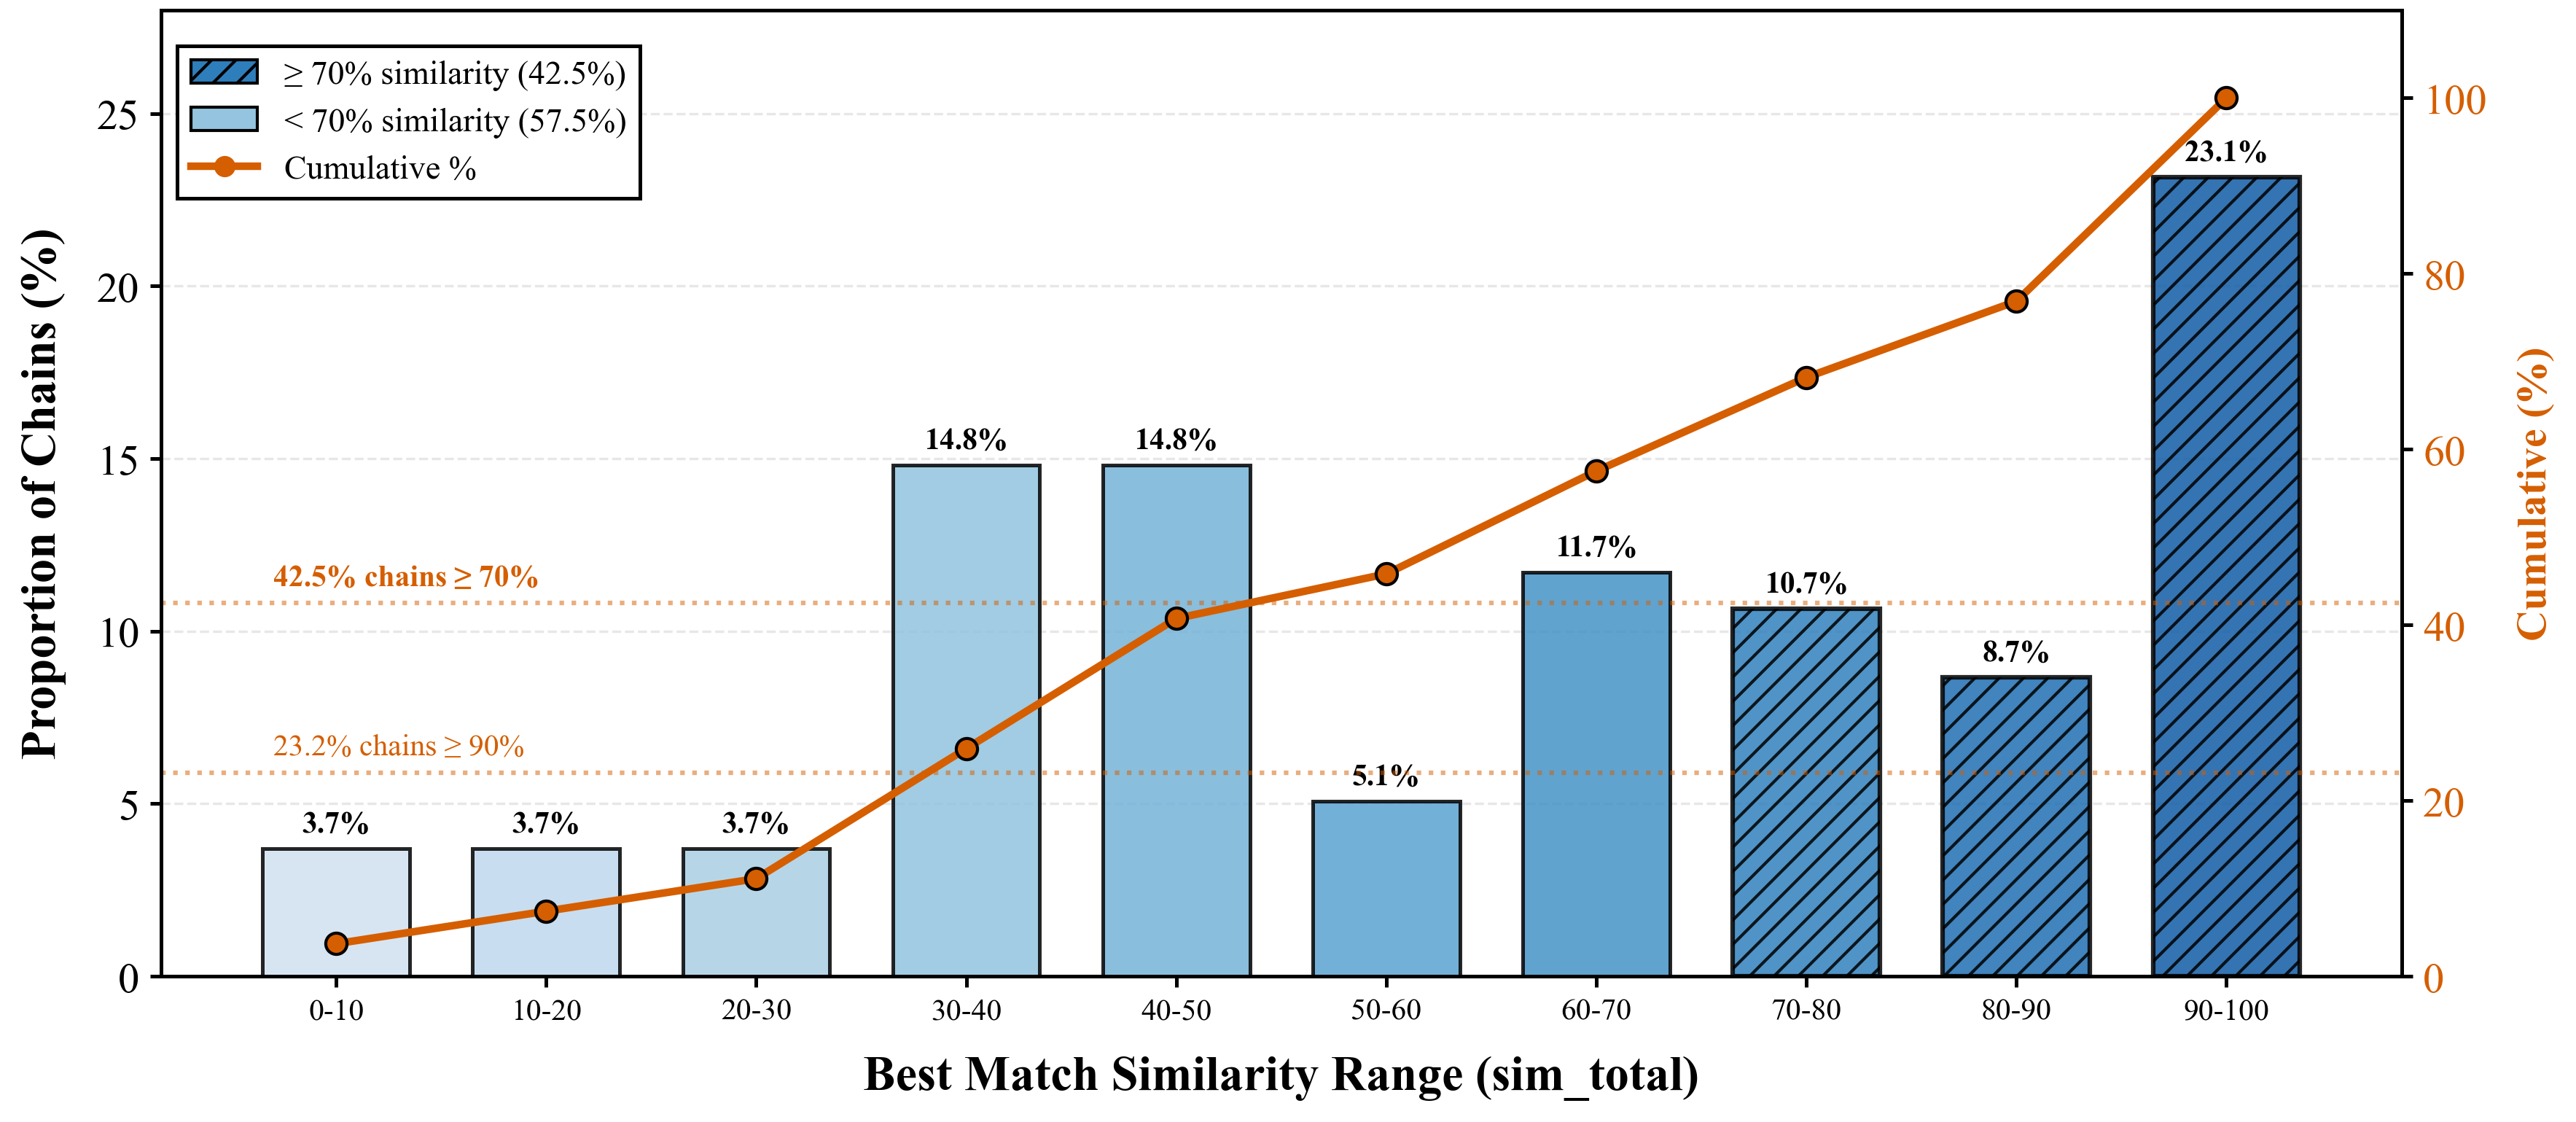
\includegraphics[width=0.98\textwidth]{figures/figure1_similarity_distribution.png}
\caption{Distribution of Best-Match Similarity (sim\_total) Across 1,320,030
Trip Chains}
\end{figure}

Figure~1 reveals a bimodal distribution: the largest concentration falls in
the 90--100\% bin (23.1\%), while two nearly equal secondary modes appear at
30--40\% and 40--50\% (14.8\% each), separated by a valley at 50--60\%
(5.1\%). Overall, 42.5\% of chains achieve sim\_total $\geq$ 0.70, confirming
that OTP generates at least one behaviorally close alternative for a
substantial share of trips, while the remaining 57.5\% highlights the scope
for model-based re-ranking.

\subsection{Model Estimation Results}

\subsubsection{MNL: Pooled and User-Type-Specific Results}

Table~6 reports MNL estimates for the pooled sample and four
user-type-specific models. All coefficients carry expected signs---negative
for ride time, walking time, and transfers; positive for subway
inclusion---with one striking exception.

\begin{table}[htbp]
\centering
\tablefont
\begin{tabular}{|l|c|c|c|c|c|}
\hline
\headrow
\textbf{Parameter} & \textbf{Pooled} & \textbf{General} & \textbf{Youth} &
\textbf{Elderly} & \textbf{Disabled} \\
\hline
$\beta_{\mathrm{ride}}$     & $-0.034$ & $-0.045$ & $-0.078$ & $+0.108$ & $+0.028$ \\
\hline
$\beta_{\mathrm{walk}}$     & $-0.776$ & $-0.767$ & $-0.880$ & $-0.785$ & $-0.840$ \\
\hline
$\beta_{\mathrm{transfer}}$ & $-3.413$ & $-3.322$ & $-3.941$ & $-4.290$ & $-3.600$ \\
\hline
$\beta_{\mathrm{subway}}$   & $+2.394$ & $+2.161$ & $+2.376$ & $+4.641$ & $+2.715$ \\
\hline
Walk Weight    & 22.7$\times$ & 16.9$\times$ & 11.2$\times$ & 7.3$\times$ & 30.2$\times$ \\
\hline
Transfer (min) & 100.0 & 73.3 & 50.3 & 39.6 & 129.6 \\
\hline
$\rho^2$       & 0.469 & 0.459 & 0.486 & 0.582 & 0.515 \\
\hline
Hit Rate       & 62.9\% & 62.1\% & 63.8\% & 78.5\% & 73.0\% \\
\hline
\end{tabular}
\caption{MNL Parameter Estimates by User Type. p$<$0.001, p$<$0.01}
\end{table}

The most notable result in Table~6 is the positive $\beta_{\mathrm{ride}}$
for elderly users ($+0.108$, t = 17.1). Under the standard assumption of time
minimization, this coefficient should be negative; its reversal suggests that
elderly travelers prefer longer in-vehicle times, likely because longer subway
rides afford a seated, climate-controlled journey free of stair-climbing and
crowd-navigation. Consistent with this interpretation, their subway
coefficient ($\beta_{\mathrm{subway}} = +4.641$) is more than double that of
general users ($+2.161$).

At the other end of the spectrum, disabled users exhibit the highest walking
weight (30.2$\times$), implying that each minute of walking is perceived as
equivalent to roughly half an hour of in-vehicle travel. Their transfer
penalty of 129.6 minutes---nearly twice that of general users (73.3
min)---substantially exceeds the 13--18-minute range in Jara-D\'iaz et
al.'s \cite{jaradiaz2022} international meta-analysis, suggesting that
population-average estimates may severely understate the disutility faced by
mobility-impaired subgroups.

\subsubsection{Mixed Logit Results}

Mixed Logit estimation ($\rho^2$ = 0.464) yields highly significant standard
deviations for all three random coefficients (p $<$ 0.001), with the walking
weight spanning a 95\% interval of 14.0$\times$ to 36.3$\times$ (LRT $\approx$
1,040, df = 3, p $<$ 0.001). Both peak interaction terms become
non-significant once heterogeneity is accommodated (p = 0.33 and 0.86),
suggesting that apparent peak effects in MNL were proxies for unobserved
individual variation. The elderly subgroup harbors the widest within-group
heterogeneity: their transfer penalty 95\% range spans 7.9 to 76.7 minutes,
confirming that the ``elderly'' card-type label conceals enormous behavioral
diversity.

\subsubsection{Latent Class Results (K = 3)}

\begin{table}[htbp]
\centering
\tablefont
\begin{tabular}{|l|c|c|c|c|c|}
\hline
\headrow
\textbf{Parameter} & \textbf{Class 1 (8.7\%)} & \textbf{Class 2 (77.2\%)} &
\textbf{Class 3 (14.0\%)} & \textbf{Walk Wt.} & \textbf{Xfer (min)} \\
\hline
$\beta_{\mathrm{ride}}$     & $+0.252$  & $-0.077$ & $+1.166$  & ---              & ---    \\
\hline
$\beta_{\mathrm{walk}}$     & $-1.123$  & $-0.730$ & $-10.000$ & 9.5$\times^{2}$  & ---    \\
\hline
$\beta_{\mathrm{transfer}}$ & $-10.000$ & $-3.272$ & $-10.000$ & ---              & 42.5$^{2}$ \\
\hline
$\beta_{\mathrm{subway}}$   & $+8.120$  & $+2.022$ & $+10.000$ & ---              & ---    \\
\hline
\end{tabular}
\caption{Latent Class Utility Parameters. $^{2}$ = Class 2 only. All p$<$0.001}
\end{table}

The BIC-optimal three-class solution reveals a strikingly interpretable
segmentation. Class 1, ``Accessibility-Priority Travelers'' (8.7\%), is
characterized by positive ride-time valuation ($+0.252$), boundary-level
transfer aversion ($\beta_{\mathrm{transfer}} = -10.0$), and dominant subway
preference ($\beta_{\mathrm{subway}} = +8.12$). The concomitant variable for
elderly card type yields an odds ratio of 22.0---yet only 61\% of elderly
users map to this class; the remaining 39\% split between Mainstream (26\%)
and Extreme (13\%) classes. The resulting Cram\'er's V of 0.685 indicates that
card type and behavioral class are strongly correlated but far from
identical---administrative demographics are a useful starting point for
personalization, not an endpoint.

Class 2, the ``Mainstream Travelers'' (77.2\%), exhibits rational trade-offs
with a walking weight of 9.5$\times$ and transfer penalty of 42.5 minutes.
Class 3, ``Extreme Subway Loyalists'' (14.0\%), has every coefficient at or
near its estimation boundary. The model achieves $\rho^2$ = 0.474 with
excellent generalization: training and test Hit Rates (67.67\% vs.\ 67.43\%)
differ by 0.24 percentage points, ruling out overfitting.

\subsection{Multi-Model Comparison}

\begin{table}[htbp]
\centering
\tablefont
\begin{tabular}{|l|c|c|c|c|}
\hline
\headrow
\textbf{Model} & \textbf{Parameters} & \textbf{Hit Rate} & \textbf{Mean Prob} & $\boldsymbol{\rho^2}$ \\
\hline
LC (K=3)      & 24               & 67.4\% & 60.3\% & 0.474 \\
\hline
LightGBM Full & $\sim$313 trees  & 66.2\% & 40.4\% & ---   \\
\hline
MNL (Pooled)  & 6                & 66.0\% & 60.0\% & 0.469 \\
\hline
Mixed Logit   & 9                & 65.9\% & 60.7\% & 0.464 \\
\hline
LightGBM Core & $\sim$596 trees  & 65.8\% & 43.5\% & ---   \\
\hline
\end{tabular}
\caption{Model Performance Comparison (Test Set: 82,351 Chains)}
\end{table}

\begin{figure}[htbp]
\centering
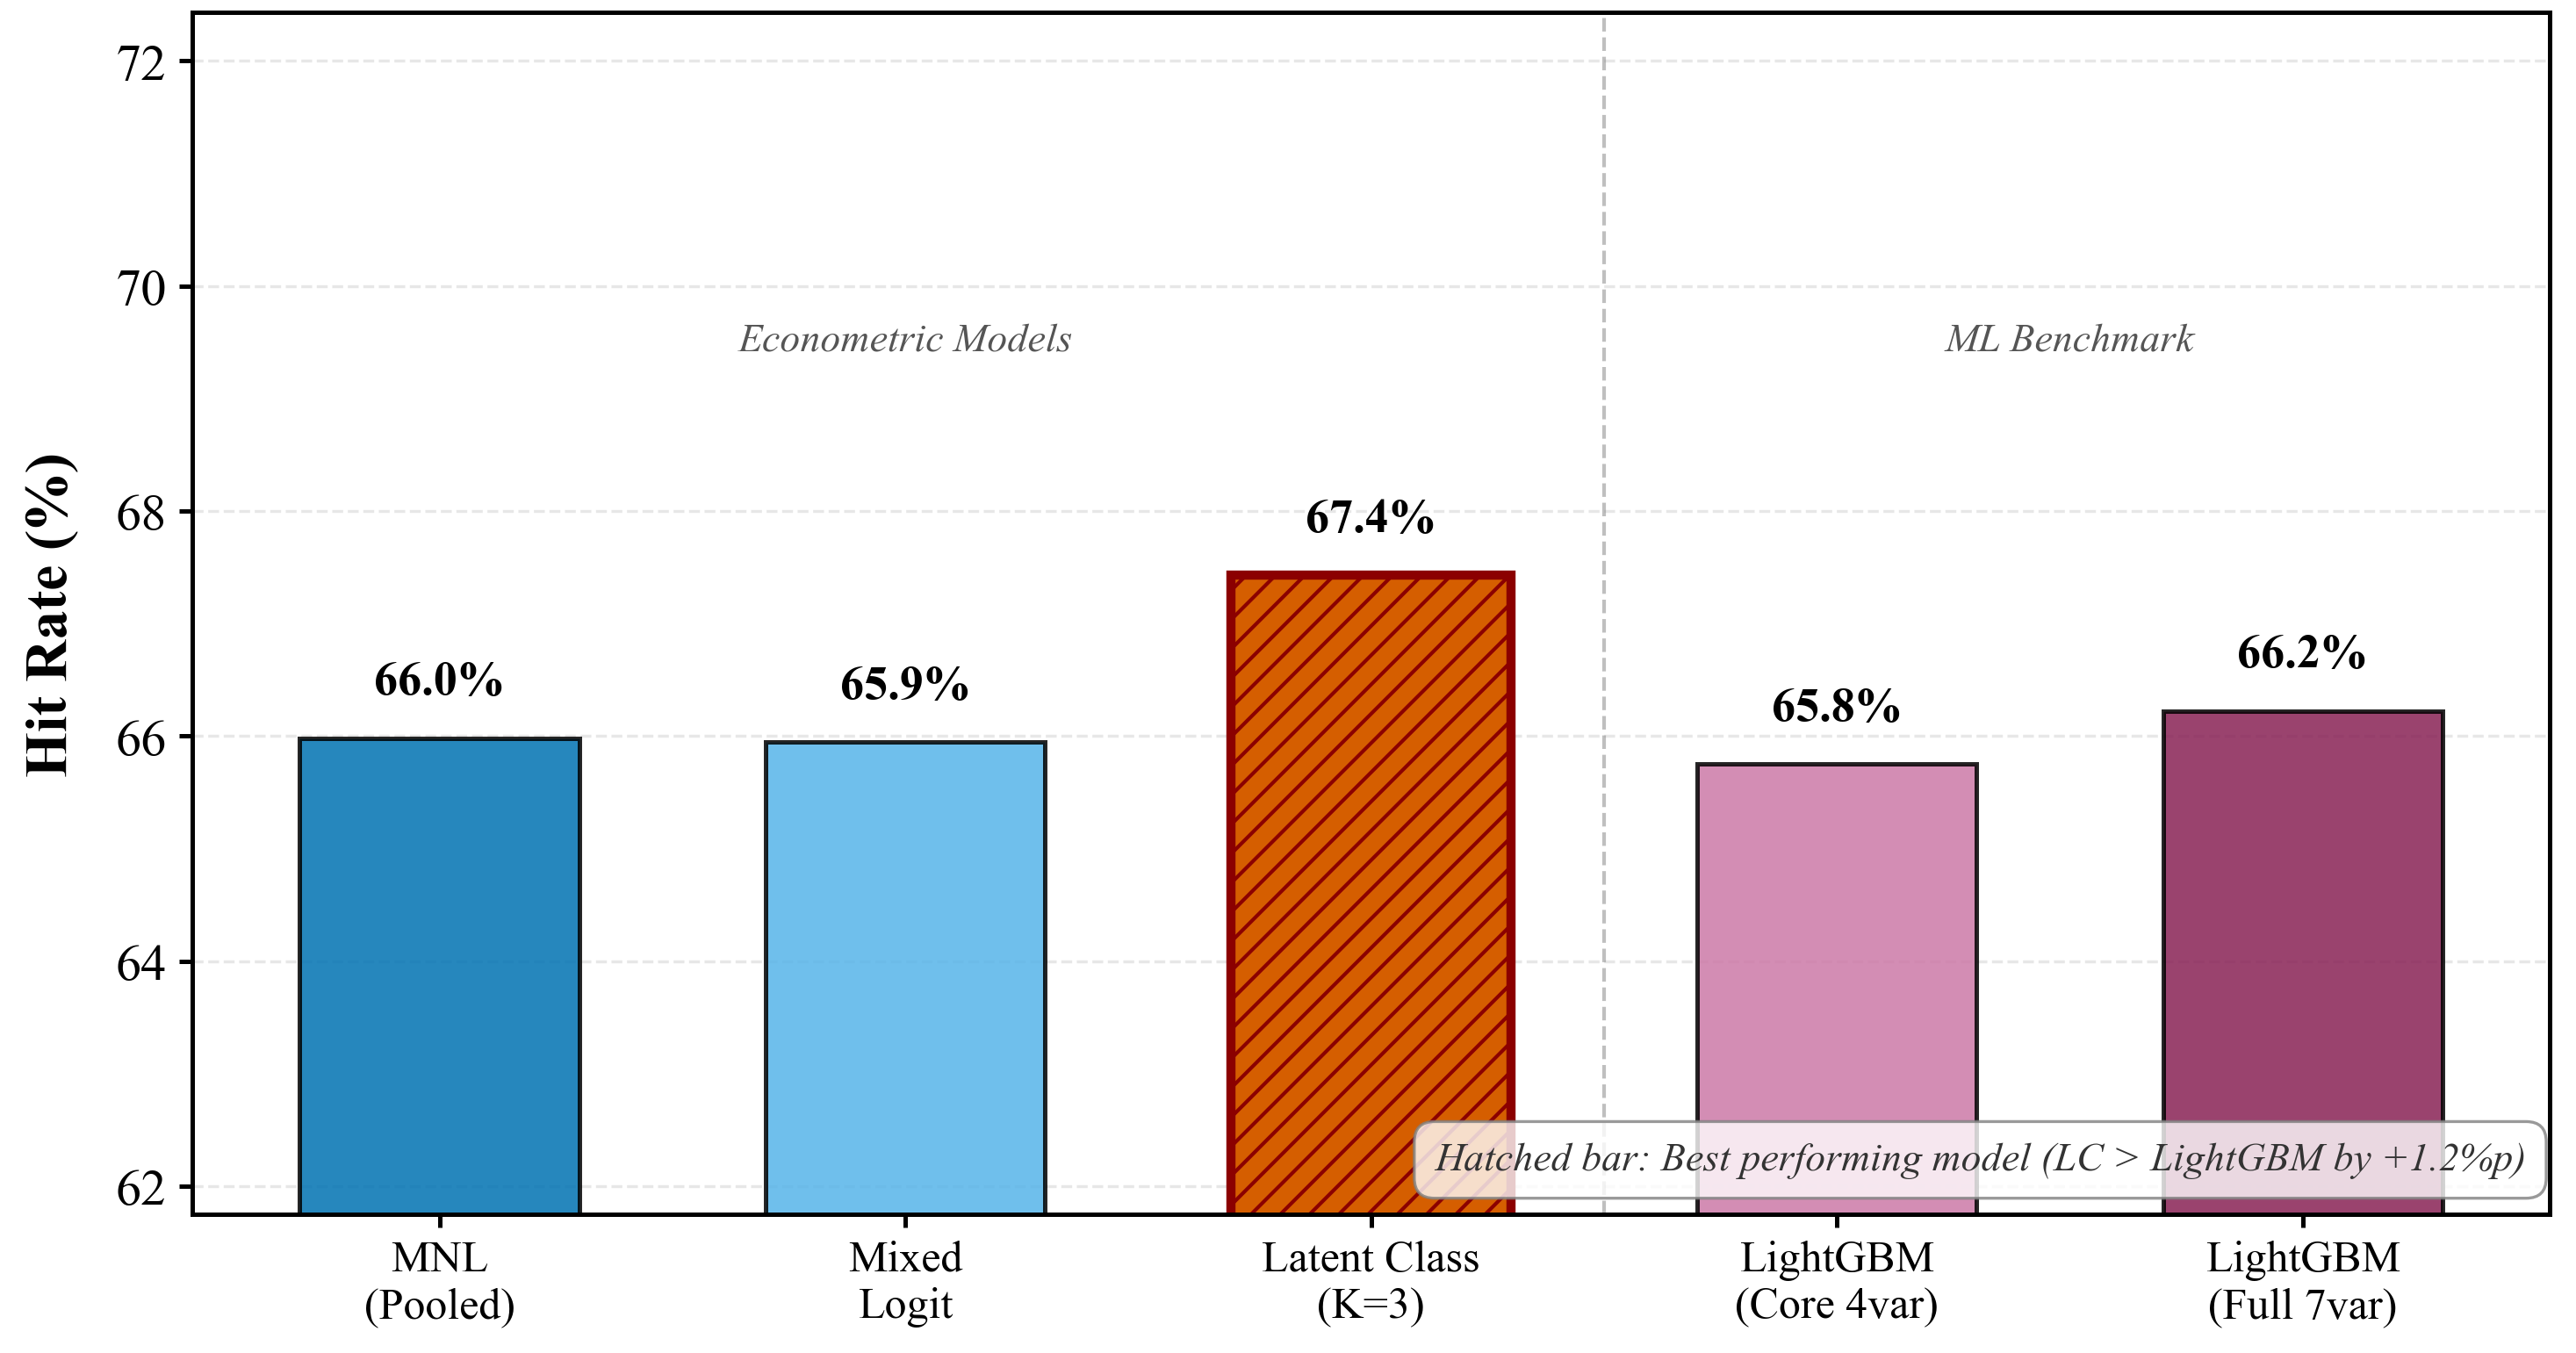
\includegraphics[width=0.9\textwidth]{figures/figure2_model_comparison.png}
\caption{Model Hit Rate Comparison on the Hold-Out Test Set}
\end{figure}

The Latent Class model leads at 67.4\%, followed by LightGBM Full (66.2\%),
MNL (66.0\%), Mixed Logit (65.9\%), and LightGBM Core (65.8\%). That a
24-parameter economic model outperforms a gradient boosting ensemble
demonstrates that choice-set structure---the constraint that exactly one
alternative is chosen from a defined set---carries substantial predictive
information that LightGBM forfeits by treating alternatives independently.
Equally striking is plain MNL, whose 66.0\% represents 99.7\% of LightGBM
Full's performance with just six parameters. The tight 1.6 percentage point
band suggests a natural accuracy ceiling imposed by unobserved factors.

\subsubsection{Cross-Validation via SHAP}

\begin{figure}[htbp]
\centering
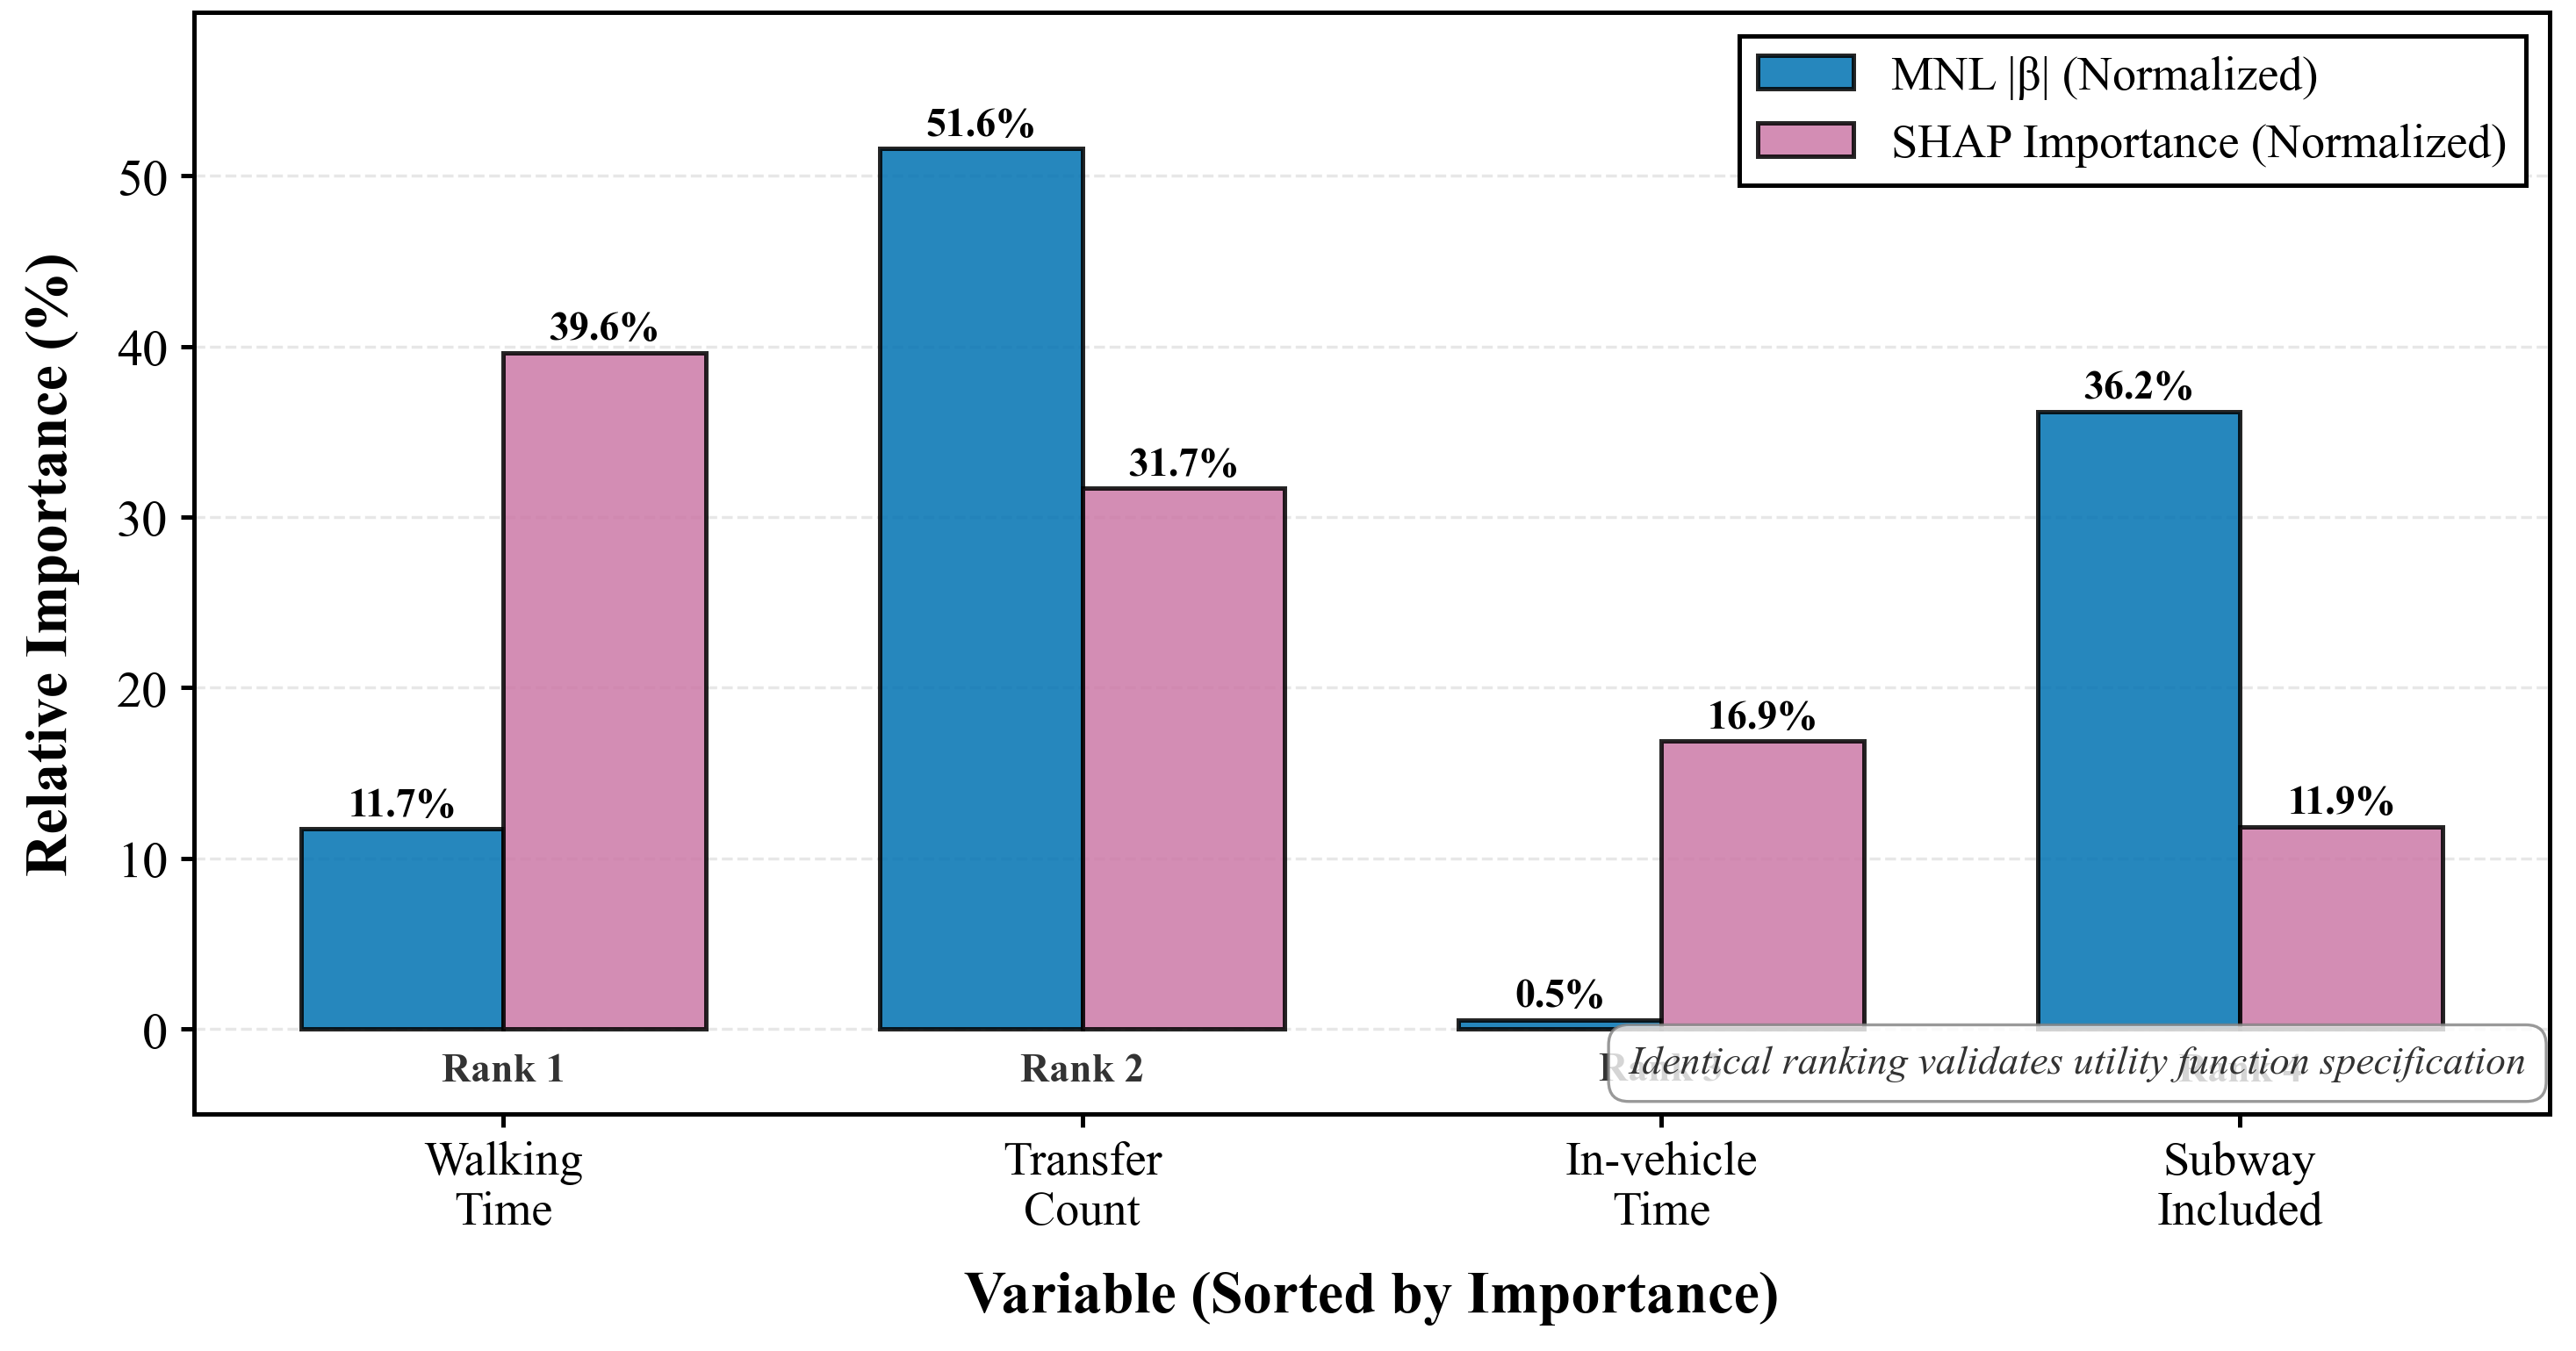
\includegraphics[width=0.9\textwidth]{figures/figure3_shap_validation.png}
\caption{SHAP Variable Importance vs.\ MNL $|\beta|$ Rankings (Spearman $\rho$ = 1.0)}
\end{figure}

SHAP importance scores from LightGBM yield perfect rank concordance with
absolute MNL coefficients (Spearman $\rho$ = 1.0): walking time ranks first,
followed by transfers, in-vehicle time, and subway indicator. This
theory-driven/data-driven agreement strongly supports our utility
specification; $D_{\mathrm{peak}}$'s near-zero SHAP value (0.002) further
confirms that peak-hour effects do not materially shape route choice in Seoul.
